% !TeX root =  main.tex

\chapter{Polynomial and Rational Functions}

\section{Quadratic Functions}
\begin{definition}
  A function $f(x)=ax^2+bx+c$ with $a\ne 0$ is called a \textbf{quadratic function}. Its graph is called a \textbf{parabola}. By completing the square (let $h=-\dfrac{b}{2a}$ and $k=f(h)$), a quadratic function can written in the \textbf{standard form} (or \textbf{vertex form}): $f(x)=a(x-h)^2+k$. The vertical line $x=-\dfrac{b}{2a}$ (or $x=h$) is called the \textbf{axis of symmetry}. The \textbf{vertex} $(h,k)$ is the intersection of the axis of symmetry and the parabola.
\end{definition}
\begin{note}
  The $y$-intercept of a quadratic function is $(0, f(0))$. The $x$-coordinates of $x$-intercepts are the zeros (or roots) of the function $f$, that is the solutions of the equation $f(x)=0$.
\end{note}

\begin{example}
  Find the vertex form of the quadratic function $f(x)=2 x^{2} + 4 x + 1$ and determine the vertex, axis of symmetry, $x$-intercepts, and $y$-intercept of the function.
\end{example}

\begin{note}
  \begin{itemize}
    \item A quadratic function $f(x)=ax^2+bx+c$ can be obtained from $y=x^2$ by a combination of vertical stretch by a factor $|a|$, a vertical reflection if $a<0$, a vertical shift of $k$ units, and a horizontal shift of $h$ units.
    \item The domain of a quadratic function is $(-\infty, \infty)$.
    \item If $a>0$, then the parabola opens upward, the function has a global (absolute) minimum $f\left(-\dfrac{b}{2a}\right)$ (or $f(h)$), and the domain of the function is $\bigg[f\left(-\dfrac{b}{2a}\right), \infty\bigg)$.
    \item If $a<0$, then the parabola opens downward, the function has a global (absolute) maximum $f\left(-\dfrac{b}{2a}\right)$ (or $f(h)$), and the domain of the function is $\bigg(-\infty,f\left(-\dfrac{b}{2a}\right)\bigg]$.
  \end{itemize}
\end{note}
\newpage

\begin{example}
 Find the vertex form equation for the quadratic function $g$ in figure below as a transformation of $f(x)=x^2$, and then simplify the equation into general form.

 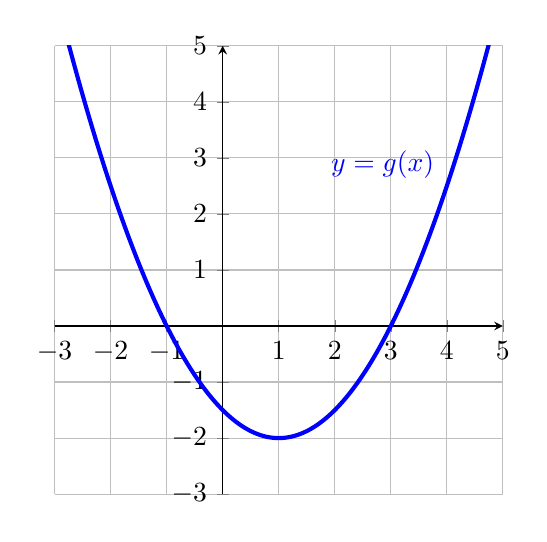
\begin{tikzpicture}
  \begin{axis}[
  axis lines=middle,
  unit vector ratio=1 1,
  ymajorgrids=true,
  xmajorgrids=true,
  xmin=-3,
  xmax=5,
  ymin=-3,
  ymax=5,
  xtick={-10,-9,...,10},
  ytick={-6,-5,...,6},]
  \addplot[blue, line width=1.5pt, smooth,samples=100,domain=-3:5] {1/2*(x-1)^2-2} node[pos=0.8, above left] {$y=g(x)$};
  \end{axis}
  \end{tikzpicture}
\end{example}

\begin{example}
  Find the domain and range of each function.\\
  \begin{enumerate*}
    \item $f(x)=3x^2+6x-5$.
    \item $f(x)=-2x^2+4-1$.\hfill\null
  \end{enumerate*}
\end{example}

\begin{example}
  A backyard farmer wants to enclose a rectangular space for a new garden within her fenced backyard. She has purchased 80 feet of wire fencing to enclose three sides, and she will use a section of the backyard fence as the fourth side.
\end{example}

\newpage

\begin{example}
  A local newspaper currently has 84,000 subscribers at a quarterly charge of \$30. Market research has suggested that if the owners raise the price to \$32, they would lose 5,000 subscribers. Assuming that subscriptions are linearly related to the price, what price should the newspaper charge for a quarterly subscription to maximize their revenue?
\end{example}

\begin{example}
  A ball is thrown upward from the top of a 40 foot high building at a speed of 80 feet per second. The ball's height above ground can be modeled by the equation \(H(t)=-16t^2+80t+40\).
\begin{enumerate}
  \item When does the ball reach the maximum height?
  \item What is the maximum height of the ball?  
  \item When does the ball hit the ground?
\end{enumerate}
\end{example}

\newpage

\section*{Exercise}

\begin{exercise}
  For each of the following functions,
  \begin{enumerate*}[label={()\alph*)}]
    \item $f(x)=x^2-4x+1$,
    \item $f(x)=-2x^2-4x+1$,\hfill\null
  \end{enumerate*}
  \begin{enumerate}
    \item write the function in vertex form,
    \item find the axis of symmetry,
    \item find the vertex,
    \item find the $y$-intercept,
    \item find the $x$-intercepts if they exist,
    \item find the domain and range,
    \item find the global maximum or minimum if it exist.
  \end{enumerate}
\end{exercise}

\begin{exercise}
  Find the vertex form equation for the quadratic function $f$ in figure below, and then simplify the equation into general form.
 
  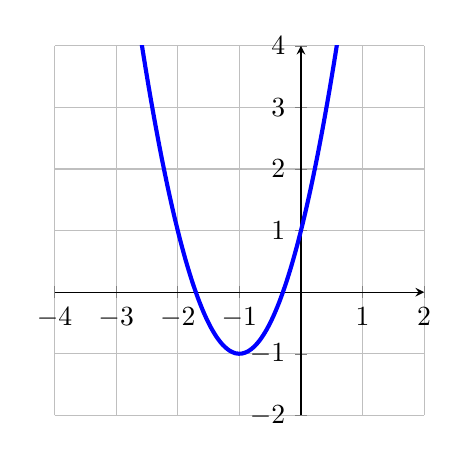
\begin{tikzpicture}
   \begin{axis}[
    width=0.6\textwidth,
   axis lines=middle,
   unit vector ratio=1 1,
   ymajorgrids=true,
   xmajorgrids=true,
   xmin=-4,
   xmax=2,
   ymin=-2,
   ymax=4,
   xtick={-10,-9,...,10},
   ytick={-6,-5,...,6},]
   \addplot[blue, line width=1.5pt, smooth,samples=100] {2*(x+1)^2-1} node[pos=0.2, right] {$y=f(x)$};
   \end{axis}
   \end{tikzpicture}
 \end{exercise}

\newpage

\begin{exercise}
  Find the dimensions of the rectangular parking lots producing the greatest area given that \(500\) feet of fencing will be used to for three sides.
\end{exercise}

\begin{exercise}
  A rocket is launched in the air. Its height, in meters above sea level, as a function of time, in seconds, is given by \(h(t)=-4.9t^2+229t+234\). Find the maximum height the rocket attains.
\end{exercise}

\begin{exercise}
  A soccer stadium holds \(62,000\) spectators. With a ticket price of \(\$11\), the average attendance has been \(26,000\). When the price dropped to \(\$9\), the average attendance rose to \(31,000\). Assuming that attendance is linearly related to ticket price, what ticket price would maximize revenue?
\end{exercise}

\newpage

\section{Power and Polynomial Functions}

\section{Graphs of Polynomial Functions}

\section{Dividing of Polynomials}

\section{Zeros of Polynomials}

\section{Rational Functions}

\section{Polynomial and Rational Inequalities}



